\chapter{Introduction}
\label{ch1}

%%%%% https://cerncourier.com/a/pushing-the-precision-frontier/
% https://home.cern/news/news/physics/why-precision-luminosity-measurements-matter
Particle physics is the branch of physics that focuses on studying the fundamental particles and forces that make up matter and radiation in the universe. The Standard Model classifies the fundamental particles and their interactions as fermions, which are matter particles, and bosons, which are force-carrying particles. High-energy particle accelerators are used to study these interactions by measuring various parameters and properties of the particles produced during collisions. This chapter provides a brief overview of elementary particles, particle colliders, and the measurement of their performance. It emphasizes the concepts and definitions necessary for understanding this thesis project.

\section{Particle Physics and The Standard Model}

The universe is composed of several different particles. Atoms consist of negatively charged electrons $(e^{-})$, which are in a bound state, orbiting a central nucleus that is composed of electrically neutral neutrons $(n)$ and positively charged protons $(p)$. The electrostatic attraction between opposite charges binds the electrons to the nucleus, while the protons and neutrons are held together by the strong nuclear force. The fundamental interactions of particle physics are completed by gravity and the weak force. The weak force drives nuclear decays $\beta$ and nuclear fusion, whereas gravity, despite being extremely weak, is universally attractive and, thus, shapes the large-scale structure of the universe.
While this is a simple physical model, at higher energy scales, more complex structures are observed, leading to the discovery of 17 fundamental particles that make up our entire universe. These particles are categorized into two groups: fermions, which possess a spin of $1/2$, and bosons, which have an integer spin. \cite{thomson_2013}.\\

Matter is composed of fermions, which consist of twelve fundamental particles classified into two types: leptons and quarks. These particles are organized into three generations, with each higher generation member having a greater mass than its corresponding particle in the previous generation. The group of six leptons includes three charged particles: electron ($e$\textsuperscript{-}), muon (${\mu}$\textsuperscript{-}), and tau (${\tau}$\textsuperscript{-}), as well as their corresponding neutrinos: electron-neutrino ($\nu_{e}$), muon-neutrino ($\nu_{\mu}$), and tau-neutrino ($\nu_{\tau}$). On the other hand, quarks can only be found in hadrons. The quark group consists of the up quark ($u$), down quark ($d$), charm quark ($c$), strange quark ($s$), top quark ($t$), and bottom quark ($b$) \cite{griff,thomson_2013}. The properties of these twelve particles are summarized in Table \ref{tab:table1}.

\begin{table}[h!]
	\begin{center}
%\centering
	\caption[The twelve fundamental fermions and their properties]{Classification and properties of the twelve fundamental Fermions divided between Quarks and Leptons\cite{thomson_2013}.}
		\label{tab:table1}
		\begin{tabular}{lllrcllrc}
                                                                                & \multicolumn{4}{c}{\textbf{Leptons}}                                                                     & \multicolumn{4}{c}{\textbf{Quarks}}                                                \\ 
%\cline{2-9}
 \midrule[1.1pt]
                            \multicolumn{1}{c}{Generation }& \multicolumn{2}{c}{Particle } & \multicolumn{1}{c}{\textit{Q}} & mass/GeV                          & \multicolumn{2}{c}{Particle} & \multicolumn{1}{c}{\textit{Q}} & mass/GeV  \\ 
\hline
\multirow{2}{*}{\begin{tabular}[c]{@{}l@{}}First\end{tabular}}  & electron & ($e$\textsuperscript{-})                 & -1                             & 0.0005                            & down    & ($d$)                & -1/3                           & 0.003     \\
                                                                                & $e$-neutrino & ($\nu_{e}$)                 & 0                              & \textless{}10\textsuperscript{-9} & up      & ($u$)                & +2/3                           & 0.005     \\
\multirow{2}{*}{\begin{tabular}[c]{@{}l@{}}Second\end{tabular}} & muon     & (${\mu}$\textsuperscript{-})                 & -1                             & 0.106                             & strange & ($s$)                & -1/3                           & 0.1       \\
                                                                                & $\mu$-neutrino & ($\nu_{\mu}$)                 & 0                              & \textless{}10\textsuperscript{-9} & charm   & ($c$)                & +2/3                           & 1.3       \\
\multirow{2}{*}{\begin{tabular}[c]{@{}l@{}}Third\end{tabular}} & tau      & ({$\tau}$\textsuperscript{-})                 & -1                             & 1.78                              & bottom  & ($b$)                & -1/3                           & 4.5       \\
                                                                                & $\tau$-neutrino & ($\nu_{\tau}$)                 & 0                              & \textless{}10\textsuperscript{-9} & top     &($t$)                & +2/3                           & 174      
\end{tabular}
	\end{center}
		\end{table}

Bosons serve as mediators of interactions between fermions by exchanging particles known as gauge bosons. The electromagnetic force is carried by the photon $\gamma$, while the weak force is mediated by $W^{\pm}$ and $Z^{0}$ bosons and the strong force by gluons $g$ \cite{thomson_2013}. A scalar boson, the Higgs boson, is also present and plays a crucial role in providing mass to all fundamental particles. Table \ref{tab:table2} provides a comprehensive overview of the forces experienced by fermions.

\begin{table}[h!]
  \begin{center}
    \caption[Force experienced by the fermions]{Force experienced by the fermions \cite{thomson_2013}.}
    \label{tab:table2}
    \begin{tabular}{l c c c c}
    &    &  \textbf{Electromagnetic} & \textbf{Weak} & \textbf{Strong}\\
      \midrule[1.1pt]
      \multirow{2}{*}{Leptons} & ${e}$\textsuperscript{-} \hspace{0.3cm}  ${\mu}$\textsuperscript{-} \hspace{0.3cm} ${\tau}$\textsuperscript{-} & \checkmark & \checkmark & \\ % <-- Combining 2 rows with arbitrary with (*) and content 12
      & $ \nu_{e} $ \hspace{0.3cm}  $\nu_{\mu}$ \hspace{0.3cm} $\nu_{\tau}$  &  & \checkmark\\ % <-- Content of first column omitted.
      \hline
      \multirow{2}{*}{Quarks} & $u$ \hspace{0.5cm}  $c$\hspace{0.5cm} $t$ & \checkmark & \checkmark& \checkmark\\
      & $d$ \hspace{0.5cm}  $s$\hspace{0.5cm} $b$ & \checkmark & \checkmark & \checkmark\\

    \end{tabular}
  \end{center}
\end{table}

All the particles mentioned are described by the Standard Model of particle physics (SM), which is the best theoretical model to date for providing a successful description of experimental data. However, most of this data comes from particle colliders since these particles can only be produced and studied through collisions at high energy.

\section{Particle Colliders and production cross section}

Particle physics has experienced significant advances in recent times due to high-energy particle accelerators. These accelerators function as powerful microscopes capable of examining the tiniest inner structures of matter and their constituent particles like electrons, protons, neutrons, neutrinos, and quarks. Additionally, these accelerators have the potential to solve questions about new fundamental components of the universe that remain undiscovered, including dark matter and dark energy.\\

Particle colliders produce and accelerate beams of charged particles at relativistic speeds using electromagnetic fields. When the beams collide at high energies, individual interactions known as events are generated. These collisions produce several particles (such as the Higgs boson),these particles  can not be observed directly because immediately they transform or decay into other particles. They are measured and identified by a wide range of experiments (particle detectors), whose technologies, techniques and designs are based on the properties of the particles and on the nature of their interactions with matter \cite{thomson_2013}.\\

In general, particle detector is typically constructed as a cylindrical or polygonal barrel section, oriented parallel to the incoming colliding beams. Two flat end caps seal the cylindrical structure, ensuring nearly complete solid angle coverage all the way down to the beam pipe. This detector comprises multiple layers, each designed to detect the different particles generated during collisions \cite{thomson_2013}.\\

Particle colliders are evaluated based on two important measures, which are the energy of the particle beams and the rate at which particles collide (luminosity). The amount of energy that is available to create new particles and study their properties is particularly significant because it determines the range of particles that can be detected or investigated. During experiments, particles are accelerated and directed towards each other, and when they collide, they produce new particles and interactions that can be analyzed by scientists.\\

Colliding beam machines are capable of achieving significantly higher energies at the point where the beams intersect and scatter. When the particles in the beams have equal energy and opposite momentum (equal mass), the experiment occurs in the center-of-mass (CM) frame. This allows for the entire energy delivered by the accelerator to be utilized in generating high-mass particles \cite{undergraduate_accelerators_chapter}. In particle physics, the Lorentz invariant quantity $s$ represents the square of the total incoming energy and is defined as:

\begin{equation}
s = \left ( \sum_{i = 1,2}^{}E_{i} \right )^{2}-\left ( \sum_{i = 1,2}^{}p_{i} \right )^{2}c^{2}
\end{equation}
Where  \textbf{$p$} and $E$ are the momenta and the energy of each incoming particle respectively.In the center-of-mass (CM) frame, where the momenta of the particles are equal and opposite, the second term in the equation for the Lorentz invariant quantity ($s$) disappears, leaving only $s = 4E^2$.\\

The second important parameter used to evaluate the performance of colliders is luminosity, which measures the accelerator's ability to produce the necessary number of interactions. It is determined by the proportionality factor between the quantum mechanical probability for the interaction (known as the cross section) and the number of events for a specific physics process per second ($R$) \cite{ref_lib_vol3}.\\

The technical meaning of "cross section" in particle physics is quite different from its common usage, while "cross section" typically refers to a slice of an object, in particle physics, it often refers to the probability that two particles will collide and react in a specific manner. When two beams cross in a particle accelerator, a variety of different processes can occur and  the cross section of a given process depends on the type and energy of the colliding particles.
At the Large Hadron Collider (LHC), certain particles such as  $W^{\pm}$ and $Z^{0}$ bosons have large cross sections , making their observation more frequent, while the production of a Higgs boson has a much lower cross section, making it more difficult to produce \cite{thomson_2013}.\\

To explain this concept more clearly, let's consider a simple scenario where a beam of particles of type $a$ passes through a region of space that contains particles of type $b$. The interaction rate between the two types of particles depends on the number of particles per unit volume of type $b$, denoted as $n_{b}$, and the flux of the incident particles, denoted as $\phi_{a}$. The rate of interaction per target particle of type $b$ can be expressed as follows \cite{thomson_2013}:

\begin{equation*}
  r_{b}=\sigma \phi_{a}
\end{equation*}

The essence of fundamental physics can be encapsulated in the interaction cross section, denoted by $\sigma$. This parameter, which is measured in area units, represents the likelihood that an interaction will occur between an incident particle and a target particle. It's helpful to imagine each target particle as having an effective cross-sectional area, and the interaction cross section as representing that area. Figure \ref{cross_section}(a) shows an illustration of this concept, where an incident particle of type $a$ moves with velocity $v_{a}$ through a region of area $A$ that contains target particles of type $b$ with velocity $v_{b}$ moving in the opposite direction. The value of the interaction cross section is determined by the underlying quantum mechanical probability of interaction and is fundamental to understanding the behavior of particles in collisions. \cite{thomson_2013}

\begin{center}
  \begin{figure}[h!]
    \centering
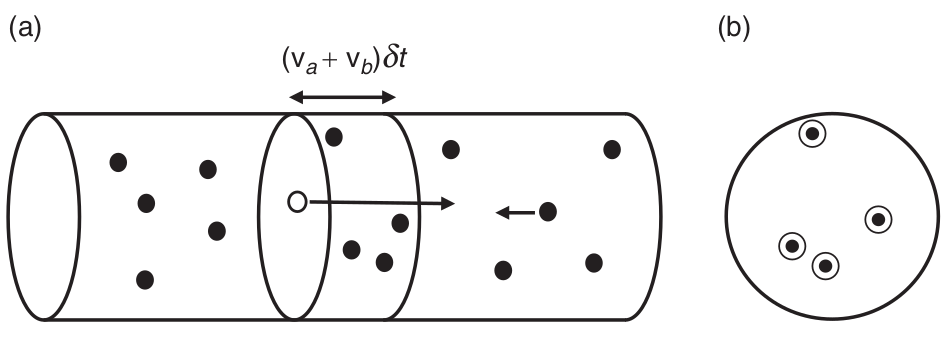
\includegraphics[scale=.35]{Chapter1/cross_section.png} 
 \caption[Cross section illustration]{Left hand (a): single incident particle of type $a$ traversing a region containing particles of type $b$. Right-hand plot (b): projected view of the region traversed by the incident particle in time $\delta t$ \cite{thomson_2013}.}
    \label{cross_section}
  \end{figure}
\end{center}

To understand the probability of an interaction between particles of types $a$ and $b$, imagine that in a time interval $\delta t$, particle $a$ passes through a region containing $\delta N= nb(v_{a}+v_{b}) A \delta t$ particles of type $b$. The probability of interaction can be obtained by dividing the effective total cross-sectional area of the $\delta N$ particles by the area $A$. This can be thought of as the probability that the incident particle passes through one of the regions of area $\sigma$ drawn around each of the $\delta N$ target particles, as shown in Figure \ref{cross_section}(b). So the cross section for a particular process is defined as the effective target area for that process and has units of area, more formally is expresed as \ref{cross} \cite{thomson_2013}.

%For a beam of particles of type $a$ with number density $n_{a}$ confined to a volume $V$, the total interaction rate can be expressed as $\text{rate}=(n_{a}v)(n_{b}V) \sigma = \phi N_{b} \sigma$, where $v$ is the velocity of the beam particles, $N_{b}$ is the number of target particles per unit volume, and $\phi$ is the flux of incident particles per unit area per unit time. The cross section for a particular process is defined as the effective target area for that process and has units of area, more formally is expresed as \cite{thomson_2013}:
\begin{equation}
\sigma=\frac{\text{number of interaction per unit time per target particle}}{\text{incident flux}}
\label{cross}
\end{equation}

%begin{equation}
%\sigma=\frac{\text{number of interaction per unit time per target particle}}{\text{incident flux}}
%\end{equation}

%\delta P= \frac{\delta N \sigma}{A}=\frac{n_{b}(v_{a}+v_{b})A\sigma \dela t}{A}= n_{b}v\sigma \delta t$
%where $v=v_{a}+v_{b}$. The interaction rate for each particle of type $a$ is $r_{a}= \frac{dP}{dt}= n_{b} v\sigma$.
%For a beam of particles of type $a$ with number density $n_{a}$ confined to a volume $V$, the total interaction rate is:
%$\text{rate}=r_{a}n_{a}V=(n_{b}v\sigma) n_{a}V= (n_{a}v)(n_{b}V)\sigma$

%$\text{rate}=(n_{a}v)(n_{b}V) \sigma = \phi N_{b} \sigma$

%Thus the total rate is equal to
%$\text{rate}= \text{flux} \times \text{number of target particles} \times \text{cross section}$

%More formally, the cross section for a process is defined as:
\section{Luminosity }

In experiments conducted in particle physics, the number of useful interactions (or events) is just as important as the energy. The ability of a particle accelerator to produce these interactions is measured by a parameter called instantaneous luminosity $\mathcal{L}_{inst}$. It is directly proportional to the number of events produced per second and the cross section $\sigma_{p}$ \cite{concept_of_luminosity}.

\begin{equation}
R=\mathcal{L}_{inst} \cdot \sigma_{p}
\end{equation}

Where the unit of luminosity is $cm^{-2}s^{-1}$. 

To derive a general expression for luminosity in the case of two colliding beams, we consider both beams to serve as the target and the incoming beam simultaneously. We will assume that the beams are "bunched", meaning that the particles are grouped into packets or bunches. 

\begin{center}
  \begin{figure}[h!]
    \centering
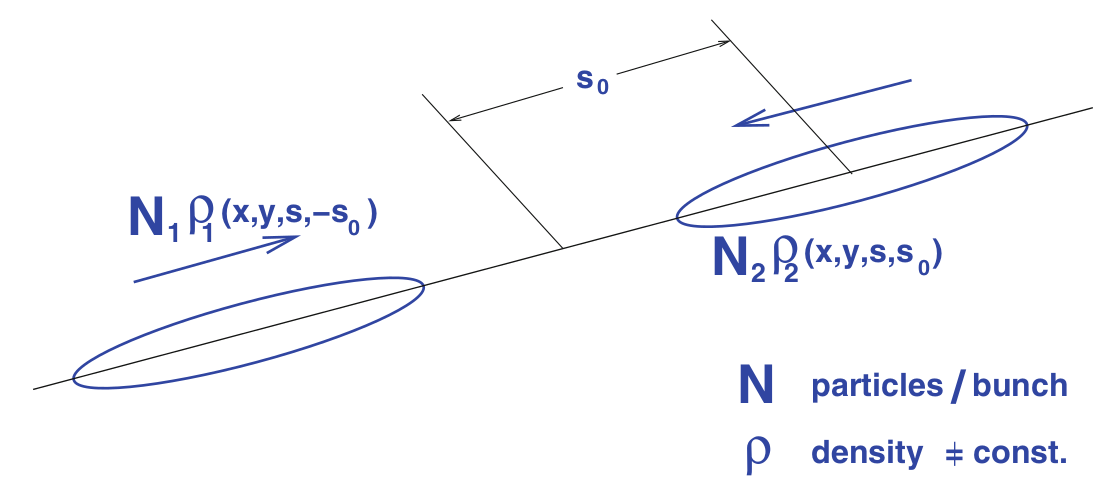
\includegraphics[scale=.25]{Chapter1/luminosity.png} 
 \caption[Colliding beam interaction]{Schematic view of a colliding beam interaction\cite{concept_of_luminosity}}
    \label{luminosity}
  \end{figure}
\end{center}

%A schematic picture is shown in Fig. \ref{luminosity}. Since the two beams are not stationary but are moving through each other, the overlap integral depends on the longitudinal position of the bunches, and therefore on time. As the beams move towards and through each other, the two beams have different distribution functions and a different number of particles in the beams \cite{concept_of_luminosity}. The overlap integral, which is proportional to the luminosity $\mathcal{L}_{inst}$, can then be written as:
 In Figure \ref{luminosity}, you can see a diagram that illustrates how two beams intersect with each other. Because these beams are not still, but rather in motion, the way they overlap depends on the time and the position of the bunches. While the beams move, they also have different distributions and numbers of particles in them \cite{concept_of_luminosity}. The luminosity $\mathcal{L}_{inst}$, which is proportional to the overlap integral, can be expressed as: 
 
\begin{equation}
  \mathcal{L}_{inst}\propto K\cdot \int\int\int \int_{-\infty}^{\infty} \rho_{1}(x,y,s,-s_{0}) \rho_{2}(x,y,s,s_{0})dxdydsds_{0}
    \label{lumi_1}
\end{equation}
 
The functions $\rho_{1}(x,y,s,-s_{0})$ and $\rho_{2}(x,y,s,s_{0})$ represent the beam density distribution at a given time. We assume that the two bunches meet at the point $s_{0} = 0$. Since the beams are in motion towards each other, we need to take into account a relativistic kinematic factor (Eq. \ref{kinematic}) by multiplying this expression.

\begin{equation}
 K = \sqrt{(\vec{v_{1}}-\vec{v_{2}})^{2}-(\vec{v_{1}}\times \vec{v_{2}})^{2}/c^{2}}
    \label{kinematic}
\end{equation}

When the bunches collide head-on and are traveling at nearly the speed of light, the relativistic kinematic factor takes on a value of 2.\\
Assuming uncorrelated densities in all planes and head-on collisions where the velocities of the two bunches are opposite $(\vec{v_{1}}=-\vec{v_{2}})$, the overlap integral can be factorized as:

\begin{equation}
  \mathcal{L}_{inst}= 2N_{b} N_{1}N_{2}f \int\int\int\int_{-\infty}^{\infty}  \rho_{1x}(x)\rho_{1y}(y)\rho_{1s}(s-s_{0})\rho_{2x}(x)\rho_{2y}(y)\rho_{2s}(s+s_{0}) dxdydsds_{0}
    \label{luminosity_2}
\end{equation}

where $N_{b}$ is the number of bunches in one beam, $N_{1}$ and $N_{2}$ are the particles per bunch and $f$ the revolution frequency.\\



%\begin{eqnarray}
%\rho_{iz}(z)= \frac{1}{\sqrt{2\pi} \sigma_{z}} exp \biggl(-\frac{z^{2}}{2\sigma_{z}^{2}} \biggr)&z=x,y&i=1,2 
%\end{eqnarray}

%\begin{eqnarray}
%\rho_{s}(s\pm s_{0})= \frac{1}{\sqrt{2\pi} \sigma_{s}} exp \biggl(-\frac{(s\pm s_{0})^{2}}{2\sigma_{s}^{2}} \biggr)
%\end{eqnarray}

Assuming Gaussian profiles in all dimensions and approximately equal bunch lengths $(\sigma_{1s}\approx \sigma_{2s})$, the equation \ref{luminosity_2} can be solved.
For a general case where $\sigma_{1x}\neq \sigma_{2x} \text{ and } \sigma_{1y}\neq \sigma_{2y}$

\begin{equation}
  \mathcal{L}_{inst}= \frac{N_{1} N_{2} N_{b}f }{2\pi \sqrt{\sigma_{1x}^{2}+\sigma_{2x}^{2}}\sqrt{\sigma_{2y}^{2}+\sigma_{2y}^{2}}}
  \label{lumi_general}
\end{equation}

For a specific case, asuming equal beams, $\sigma_{1x}= \sigma_{2x} \text{ and } \sigma_{1y}= \sigma_{2y}$:

\begin{equation}
  \mathcal{L}_{inst}= \frac{N_{1} N_{2} N_{b}f }{4\pi \sigma_{x} \sigma_{y}}
  \label{lumi_theor}
\end{equation}

This expression is widely recognized as the formula for the luminosity of two Gaussian beams that collide head-on. It reveals how the luminosity is related to the number of particles in each bunch and the size of the beams \cite{concept_of_luminosity}.\\

In practice,the integral in  \ref{luminosity_2} cannot be solved analytically because   the properties of the colliding beams are not know precisely, so a experimental technique is implemented with a dedicated machine setup to estimate the integrals, yielding a similar expression as \ref{lumi_theor}.

To determine the overall number of events, we rely on integrated luminosity, which is a measurement of the total amount of collected data. This value is crucial for evaluating the effectiveness of an accelerator and it can be expressed as: \cite{concept_of_luminosity}:

\begin{equation}
  \mathcal{L}_{int}=\int_{0}^{T} \mathcal {L}_{\text{inst}}(t') dt'
\end{equation}

Where the value of $\mathcal{L}_{inst}$ is evaluated over time $T$ (excluding possible dead time) because its intensity decreases as the number of protons reduces during the collisions of the fill. So $\mathcal{L}_{int}$ is directly related to the number of observed events as:

\begin{equation}
  \mathcal{L}_{int} \ndot \sigma_{p}= \text{number of events of interest}
\end{equation}

The integrated luminosity has units of $cm^{-2}$ and is often expressed in inverse barn ($1 barn= 10^{-24}cm^{2}$). \\

Precisely understanding luminosity is really important for physics analyses like finding new particles, measuring known particle properties, or detecting rare processes. The techniques used to figure out signal rates are quite advanced now. We understand things like detector biases, acceptances, background subtraction, and reconstruction efficiencies at levels that are better than one percent. Because of this, the accuracy of our physics measurements is mainly affected by uncertainties in luminosity. If we can increase the precision of luminosity measurements, then physicists will have a better understanding of their observations and be able to explore parts of physics that we don't currently know about \cite{luminosity_importance}.

\section{The Large Hadron Collider}
 
The Large Hadron Collider (LHC) is the world's biggest and most potent particle accelerator. It became operational on 10th September 2008 and is the most recent addition to CERN's accelerator complex. The LHC consists of a 27-kilometre ring that contains superconducting magnets, and various structures are used to accelerate particles as they move along the ring. Inside the accelerator, two particle beams travel at almost the speed of light until they collide. The beams move in opposite directions in separate beam pipes, which are kept at an ultrahigh vacuum.\\ 

Superconducting electromagnets generate a powerful magnetic field that guides the particle beams around the accelerator ring. These magnets are made up of coils of a unique electric cable that functions in a superconducting state. In this state, the cable can conduct electricity with zero resistance or energy loss. The accelerator uses a variety of magnets, including 1232 dipole magnets that are 15 metres in length and bend the beams, and 392 quadrupole magnets that are 5-7 metres long and focus the beams. Just before the collision, a different type of magnet is employed to "squeeze" the particles together, increasing the likelihood of collisions. To keep these magnets in the superconducting state, they must be cooled to a temperature as low as -271.3°C \cite{LHC}.\\

The process of generating proton beams for the LHC is a complex and multi-stage procedure. Initially, hydrogen is ionized to create protons, which are then accelerated in bunches up to 50 MeV in the Linear Accelerator 2 (LINAC2). The proton bunches are then routed through three circular accelerators: the Booster, the Proton Synchrotron (PS), and the Super Proton Synchrotron (SPS). These accelerators gradually increase the energy levels of the proton bunches to 1.4 GeV, 26 GeV, and 450 GeV, respectively \cite{lhc_complex}. Once these pre-acceleration stages are completed, the proton bunches are injected into the LHC ring where they are further accelerated to achieve energies of up to 7 TeV per bunch while circulating in opposite directions. This entire process constitutes a single LHC fill and typically involves $10^{14}$ protons that are grouped into bunches to form the proton beam. The complete CERN accelerator complex is illustrated in Figure \ref{lhc_com}.

\begin{center}
  \begin{figure}[h]
    \centering
    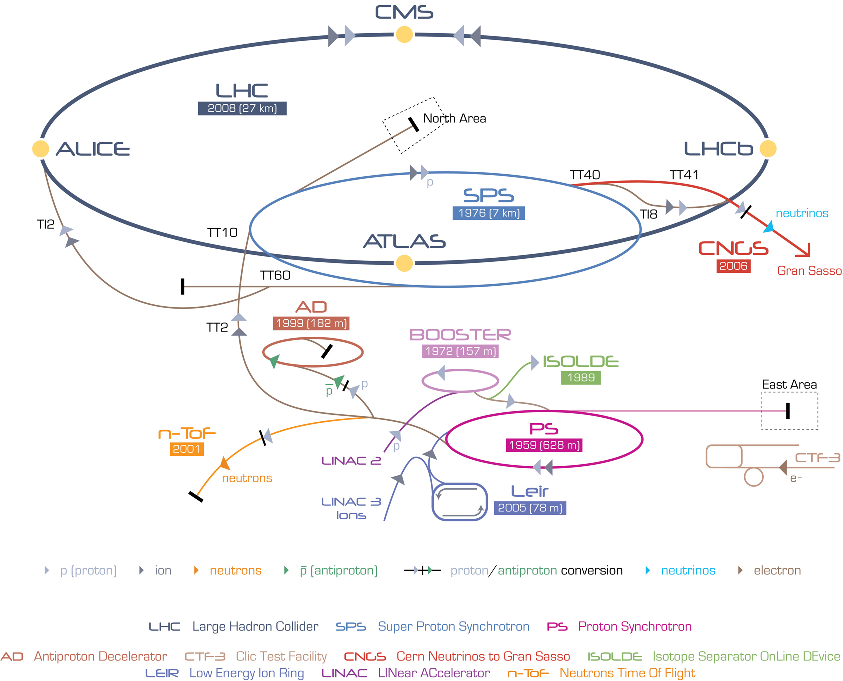
\includegraphics[scale=.45]{Chapter1/lhc_complex_fig.png}
    \caption[LHC Complex]{Diagram of the LCH complex \cite{lhc_complex}.}
    \label{lhc_com}
  \end{figure}
\end{center}

The CERN Control Centre serves as the central hub responsible for managing all controls, services, and technical infrastructure of the LHC. It directs the proton beams to collide at four distinct locations along the accelerator ring, corresponding to the positions of four particle detectors: CMS and ATLAS, which are general-purpose detectors designed to explore a broad range of Standard Model (SM) and Beyond SM (BSM) physics, while ALICE and LHCb are specialized detectors that focus on studying specific phenomena.

\section{Expected  Luminosity precision for LHC Run 3}

Since its inception in 2010 the LHC has undergone three runs and two lengthy shutdowns for maintenance and upgrades. 
Run1 began in 2010 with proton-proton collisions at a center-of-mass energy of $\sqrt{s}=\text{7 TeV}$ and concluded in 2012 at  $\sqrt{s}=\text{8 TeV}$. Run 2, which took place at $\sqrt{s}=\text{13 TeV}$, was divided into two stages; the first  occurred from 2015 to 2016, and the second part  was carried out   from 2017 to 2018, efforts are currently underway to further improve the precision of this run. Finally  Run3, which began in 2022 at $\sqrt{s}=\text{13.6 TeV}$ and is currently ongoing. This thesis project aims to contribute to the improvement of the precision of the luminosity for Run 3, where it is expected to obtain an approximate luminosity of $450 fb^{-1}$ \cite{
hl-lhc}. \\

The integrated luminosity for each of these runs and years, and their corresponding uncertainty values are presented in table \ref{lumi_values} (luminosity values encompass the duration from the start of stable beams until the beam is dumped by the LHC), also a visualization of these values measured with CMS is shown in Figure \ref{lumi_per_year_int}, which depicts the delivered luminosity versus time for each year.
% ref. TDR Bril para los 390
%separar por lumpas , poner  referencia, poner periodo en vez de Run
%-  en incertidumbre  no conocida, dejar solamente 2022
\begin{table}[h!]
    \begin{center}
    \caption[Integrated luminosity values delivered by each Run and year]{Integrated luminosity values delivered by each Run}
	\label{lumi_values}
\begin{tabular}{cccc}
\textbf{Period} & \textbf{Energy $\sqrt{s}$} & \begin{tabular}[c]{@{}c@{}}\textbf{Integrated}\\\textbf{Luminosity}\end{tabular} & \textbf{Precision}    \\ 
\toprule
Run 1(2010-2012) \cite{PCC_PAS_12_001} & 8 TeV                   & $30 fb^{-1}$                         & 2.2\%                 \\
Run 2(2015-2016) \cite{lumi_precise_2015_2016} & 13 TeV   & $45.9 fb^{-1}$                     & 1.6\%-1.2\%                \\
Run 2(2017) \cite{pas_17} & 13 TeV                                                   & $49.8 fb^{-1}$                     & 2.3\%                 \\
Run 2(2018) \cite{pas_18} & 13 TeV                                                  & $67.9 fb^{-1}$                      & 2.5\%                 \\
Run 3(2022) \cite{wikicern} & 13.6 TeV                                            & $42 fb^{-1}$                        &      -                       \\
\end{tabular}
    \end{center}
\end{table}


%%%%%%%%%%%%%%%%%%%%%%%%%%%%%%%%%%%%%%%%%%%%%%
\newpage
  \begin{center}
  \begin{figure}[ht]
    \centering
    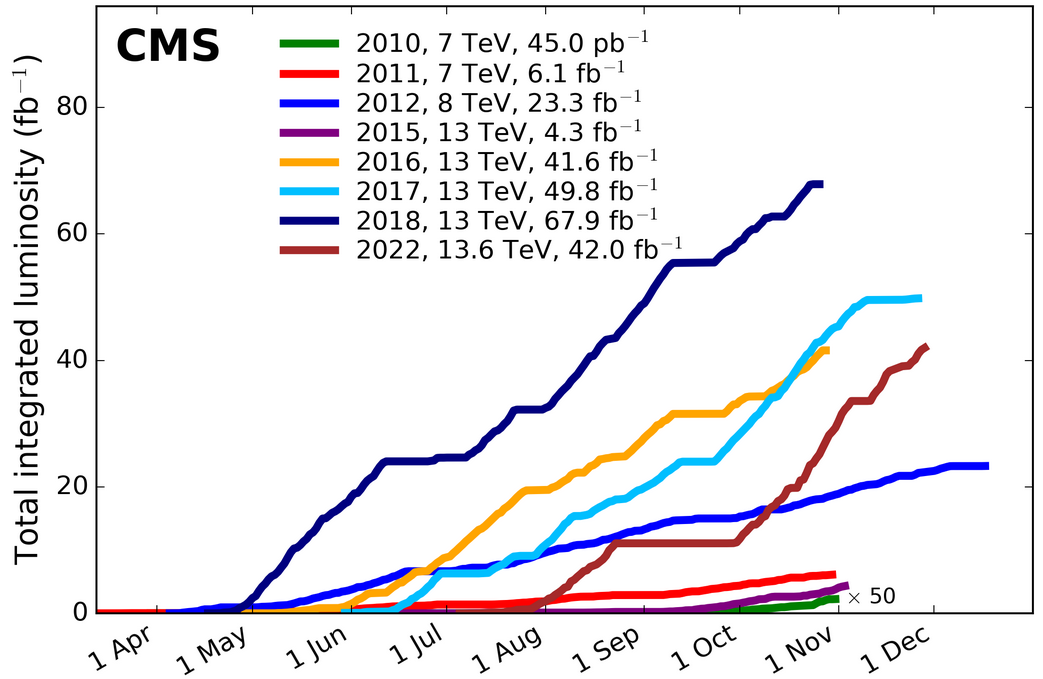
\includegraphics[scale=.35]{Chapter1/int_lumi_per_year.png}
    \caption[Delivered integrated luminosity per year]{Delivered luminosity versus time for Run-1 (2010-2012) and Run-2 (2015-2018) and Run-3 that is still ongoing . Cumulative luminosity versus day delivered to CMS during stable beams for pp collisions at nominal center-of-mass energy.  \cite{wikicern}.}
    \label{lumi_per_year_int}
  \end{figure}
    \end{center}
%% tabla con ano , luminosidad y presicion